% ======================================================================
% Contribution 3: Complete Stability Landscape
% ======================================================================

\section{Global Stability Landscape}
\label{sec:stability}

The companion TMLR paper proves a local transcritical bifurcation at
$R_0 = 1$ (Proposition~4.1) and lists three equilibrium classes
(Proposition~3.4). However, the global stability landscape---the complete
basin structure and the phase portrait across the full parameter space---
remained open. In this section, we construct a strict Lyapunov function
for the fast subsystem, classify the basins of attraction, and formalize
the hysteresis band.

\subsection{Equilibrium Classification}

\begin{definition}[Equilibrium Classes]
\label{def:equilibria}
The fast subsystem $(\delta_A, \sigma_A, \alpha_A)$ admits three
equilibrium classes:
\begin{itemize}
\item $E_0 = \{ (\delta_A, \sigma_A, \alpha_A) \in \X : \delta_A = 0,\;
  \sigma_A = 0,\; \alpha_A = 0 \}$ (the null state).
\item $E_S = \{ (\delta_A, \sigma_A, \alpha_A) \in \X :
  \delta_A > 0,\; \sigma_A = 0,\; \alpha_A \in [0,1] \}$
  (the $\sigma$-trap: high depth, zero schema coherence).
\item $E_C = \{ (\delta_A, \sigma_A, \alpha_A) \in \X :
  \delta_A > 0,\; \sigma_A = \sigma^*_A > 0,\; \alpha_A = \alpha^*_A > 0 \}$
  (the schema-coherent state: non-trivial equilibrium).
\end{itemize}
\end{definition}

Let $\alpha^*_A$ denote the non-trivial $\alpha_A$ equilibrium:
\[
\alpha^*_A = \frac{\gamma C_A}{\gamma C_A + \zeta_\alpha R_A^{\mathrm{surface}}},
\]
obtained by solving $\dot{\alpha}_A = 0$.

\subsection{Lyapunov Functions for the Fast Subsystem}

The key technical challenge is constructing Lyapunov functions that
decrease along trajectories, enabling a complete basin classification.
Because the fast subsystem is block-triangular ($\alpha_A$ dynamics do
not depend directly on $\sigma_A$, and $\delta_A$ dynamics do not depend
directly on $\alpha_A$), we can treat convergence sequentially using the
chain structure.

\begin{lemma}[$\alpha_A$ Contraction]
\label{lem:alpha-contraction}
For any fixed $\delta_A, \sigma_A \in \X$, the $\alpha_A$ ODE
\[
\dot{\alpha}_A = \gamma C_A(\delta_A, \sigma_A) (1 - \alpha_A)
- \zeta_\alpha R_A^{\mathrm{surface}}(\delta_A, \sigma_A) \alpha_A
\]
has a unique globally attracting equilibrium $\alpha^*_A$ on $[0,1]$.
The convergence is exponential with rate
$\mu_\alpha = \gamma C_A + \zeta_\alpha R_A^{\mathrm{surface}} > 0$.
\end{lemma}

\begin{proof}
The ODE is affine in $\alpha_A$: $\dot{\alpha}_A = A - B\alpha_A$ with
$A = \gamma C_A > 0$ and $B = \gamma C_A + \zeta_\alpha R_A^{\mathrm{surface}} > 0$.
The unique equilibrium is $\alpha^*_A = A/B \in (0,1]$, and the solution
$\alpha_A(t) = \alpha^*_A + (\alpha_A(0) - \alpha^*_A) e^{-Bt}$ converges
exponentially with rate $B \geq \min(\gamma C_A) > 0$ uniformly on $\X$.
\end{proof}

\begin{proposition}[Lyapunov Function for the $E_C$ Basin]
\label{prop:lyapunov-ec}
When $R_0 > 1$ and the non-trivial equilibrium $(\delta^*_A, \sigma^*_A, \alpha^*_A)$
exists, define $V_C: \X_{\mathrm{fast}} \to \R_+$ by
\[
V_C(\delta_A, \sigma_A, \alpha_A) =
\frac{1}{2}(\delta_A - \delta^*_A)^2
+ \frac{\rho P_A}{2\gamma_\sigma}(\sigma_A - \sigma^*_A)^2
+ \frac{1}{2}(\alpha_A - \alpha^*_A)^2.
\]
Then $\dot{V}_C < 0$ along trajectories of the fast subsystem for all
$(\delta_A, \sigma_A, \alpha_A)$ in the basin of $E_C$, except at the
equilibrium itself.
\end{proposition}

\begin{proof}
The time derivative of $V_C$ is
\[
\dot{V}_C =
(\delta_A - \delta^*_A) \dot{\delta}_A
+ \frac{\rho P_A}{\gamma_\sigma} (\sigma_A - \sigma^*_A) \dot{\sigma}_A
+ (\alpha_A - \alpha^*_A) \dot{\alpha}_A.
\]

For $\sigma_A$, the ODE \eqref{eq:sigma-ode} satisfies
\[
\dot{\sigma}_A = \sigma_A \bigl[ \rho P_A \alpha_A (1 - \gamma_\sigma \sigma_A)
- \epsilon_\sigma \Omega_{SL} \bigr].
\]

Using the equilibrium condition
$\epsilon_\sigma \Omega_{SL} = \rho P_A \alpha^*_A (1 - \gamma_\sigma \sigma^*_A)$:
\[
\dot{\sigma}_A = \rho P_A \bigl[ \alpha_A \sigma_A (1 - \gamma_\sigma \sigma_A)
- \alpha^*_A \sigma^*_A (1 - \gamma_\sigma \sigma^*_A) \bigr].
\]

This can be rewritten by adding and subtracting the cross-term:
\[
\begin{aligned}
\dot{\sigma}_A &= -\rho P_A \alpha_A \gamma_\sigma \sigma^*_A (\sigma_A - \sigma^*_A) \\
&\quad + \rho P_A \sigma^*_A (1 - \gamma_\sigma \sigma^*_A) (\alpha_A - \alpha^*_A) \\
&\quad + \rho P_A (\alpha_A \sigma_A - \alpha^*_A \sigma^*_A)(1 - \gamma_\sigma \sigma_A) \\
&\quad - \rho P_A \alpha_A \gamma_\sigma (\sigma_A - \sigma^*_A)^2.
\end{aligned}
\]

Substituting into $\dot{V}_C$, the coefficient of the $\sigma_A$ quadratic
term is $-\rho P_A \alpha_A \sigma^*_A \cdot (\rho P_A / \gamma_\sigma) =
-(\rho P_A)^2 \alpha_A \sigma^*_A / \gamma_\sigma < 0$ (using the weight
$w = \rho P_A / \gamma_\sigma$), and the cross-terms cancel exactly when
the $\alpha_A$ contribution is included via the $\alpha_A$ Lyapunov term.
Specifically, the cross-term
$\rho P_A \sigma^*_A (1 - \gamma_\sigma \sigma^*_A) (\alpha_A - \alpha^*_A)$
in $\dot{\sigma}_A$ combines with the $(\alpha_A - \alpha^*_A) \dot{\alpha}_A$
term. By Lemma~\ref{lem:alpha-contraction},
$(\alpha_A - \alpha^*_A) \dot{\alpha}_A = -(\gamma C_A + \zeta_\alpha
R_A^{\mathrm{surface}}) (\alpha_A - \alpha^*_A)^2$, and the residual
cross-term is bounded by the Young inequality:
\[
\begin{multlined}
\frac{\rho P_A}{\gamma_\sigma} \cdot \rho P_A \sigma^*_A
(1 - \gamma_\sigma \sigma^*_A) \\
\qquad \cdot (\sigma_A - \sigma^*_A)(\alpha_A - \alpha^*_A) \\
\qquad \leq \frac{(\rho P_A)^2 \sigma^*_A}{2\gamma_\sigma}
(\sigma_A - \sigma^*_A)^2 \\
\qquad\quad + \frac{(\rho P_A)^2 \sigma^*_A
(1 - \gamma_\sigma \sigma^*_A)^2}{2\gamma_\sigma}
(\alpha_A - \alpha^*_A)^2.
\end{multlined}
\]

With the weight $w = \rho P_A / \gamma_\sigma$, the $\sigma_A$ quadratic
coefficient remains negative. Combined with the strictly negative $\alpha_A$
quadratic term (from Lemma~\ref{lem:alpha-contraction}), we obtain
$\dot{V}_C < 0$ for all points in the $E_C$ basin, provided the trajectory
remains in the compact set $\X$ where all coefficients are bounded.
\end{proof}

\begin{proposition}[Lyapunov Function for the $E_S$ Basin]
\label{prop:lyapunov-es}
When $R_0 \leq 1$, define $V_S: \X_{\mathrm{fast}} \to \R_+$ by
\[
V_S(\delta_A, \sigma_A, \alpha_A) =
\frac{1}{2}(\delta_A - \delta^*_S)^2
+ \frac{\rho P_A}{2\epsilon_\sigma \Omega_{SL}} \sigma_A^2
+ \frac{1}{2}(\alpha_A - \alpha^*_S)^2,
\]
where $\delta^*_S$ and $\alpha^*_S$ are the $\delta_A$ and $\alpha_A$
equilibria at $\sigma_A = 0$. Then $\dot{V}_S < 0$ along all trajectories
in Regime~I, confirming that $E_S$ is globally attracting.
\end{proposition}

\begin{proof}
When $R_0 \leq 1$, the $\sigma_A$ ODE satisfies
$\dot{\sigma}_A = \sigma_A \bigl[ \rho P_A \alpha_A (1 - \gamma_\sigma \sigma_A)
- \epsilon_\sigma \Omega_{SL} \bigr]$.
Since $R_0 = \rho P_A \alpha_A / (\epsilon_\sigma \Omega_{SL}) \leq 1$,
the bracketed term is non-positive for all $\sigma_A \geq 0$, with equality
only at $R_0 = 1$ and $\sigma_A = 0$. Hence $\dot{\sigma}_A \leq 0$
globally, and $\sigma_A$ converges monotonically to $0$.

The $\delta_A$ and $\alpha_A$ subsystems, with $\sigma_A \to 0$, reduce
to their uncoupled forms, each exponentially contracting to their
respective equilibria $\delta^*_S$ and $\alpha^*_S$ (Lemma~\ref{lem:alpha-contraction}
for $\alpha_A$, and the Gompertz structure for $\delta_A$). The function
$V_S$ decreases along trajectories because each term is individually
non-increasing, confirming global attractivity of $E_S$ in Regime~I.
\end{proof}

\subsection{Basin Classification}

With the Lyapunov function established, we classify the basins of
attraction across the parameter space.

\begin{theorem}[Global Stability Landscape]
\label{thm:stability-landscape}
The parameter space $(\rho, \gamma_\sigma, \epsilon_\sigma, \Omega_{SL})$
partitions into three regimes:
\begin{itemize}
\item \textbf{Regime I ($R_0 < 1$):} $E_S$ is globally attracting.
  The $\sigma$-trap is the unique stable equilibrium. All trajectories
  converge to $E_S$ regardless of initial conditions. No positive
  $\sigma_A$ equilibrium exists.
\item \textbf{Regime II ($1 \leq R_0 < 1/(1 - \gamma_\sigma)$):}
  Bistability. $E_C$ is locally stable with basin of attraction
  containing all trajectories with $\sigma_A(0) > \sigma_{\mathrm{sep}}$,
  where $\sigma_{\mathrm{sep}}$ is the separatrix. $E_S$ remains
  locally stable for $\sigma_A(0) < \sigma_{\mathrm{sep}}$.
  The separatrix is given by the stable manifold of the saddle
  equilibrium at $\sigma_A = 0$ (the transcritical branch).
\item \textbf{Regime III ($R_0 \geq 1/(1 - \gamma_\sigma)$):}
  $E_C$ is globally attracting. The non-trivial equilibrium
  $\sigma^*_A \geq 1$ lies outside $\X$, and the numerical clamp enforces
  $\sigma_A \leq 1$. Trajectories converge to the maximal schema-coherent
  state on the boundary.
\end{itemize}
\end{theorem}

\begin{proof}
\textbf{Regime I ($R_0 < 1$).} When $R_0 < 1$, the self-derivative
$\partial \dot{\sigma}_A / \partial \sigma_A < 0$ at $\sigma_A = 0$
(Proposition~4.1 of the companion paper). The $\sigma_A = 0$ equilibrium
is stable, and the non-trivial equilibrium $\sigma^*_A$ is negative
(outside $\X$), so $E_S$ is the only stable equilibrium. By
Proposition~\ref{prop:lyapunov-es}, $V_S$ is a strict Lyapunov function
for the fast subsystem, confirming that $E_S$ is globally attracting.

\textbf{Regime II (bistability).} For $1 \leq R_0 < 1/(1 - \gamma_\sigma)$,
the transcritical bifurcation at $R_0 = 1$ has exchanged stability:
$\sigma_A = 0$ became unstable for perturbations in the positive direction,
while remaining stable for perturbations in the negative direction
($\sigma_A$ is constrained to $\X$, so only positive perturbations are
physically realizable). The non-trivial equilibrium $\sigma^*_A > 0$ is
stable. The separatrix $\sigma_{\mathrm{sep}}$ is the stable manifold of
the $\sigma_A = 0$ saddle point. Rigorously,
\[
\sigma_{\mathrm{sep}} \defeq \sup\{ \sigma \geq 0 : \omega(\sigma) = \{0\} \},
\]
where $\omega(\sigma)$ is the $\omega$-limit set of the trajectory with
initial $\sigma_A(0) = \sigma$ (and $\delta_A, \alpha_A$ at their
$E_S$ equilibrium values). This is the supremum of initial $\sigma_A$
values whose forward orbit converges to the $\sigma$-trap $E_S$.
By continuity of the flow with respect to initial conditions,
$\sigma_{\mathrm{sep}}$ is the unique point where the stable manifold
of the saddle intersects the $\sigma_A$ axis. Numerically,
$\sigma_{\mathrm{sep}}$ is the smallest positive root of the
time-reversed ODE (shooting backward from the saddle equilibrium).

\textbf{Regime III ($R_0 \geq 1/(1 - \gamma_\sigma)$).} In this regime,
$\sigma^*_A \geq 1$. The ODE would drive $\sigma_A$ toward a value
above 1, but the numerical clamp in Algorithm~3.1 of the companion paper
enforces $\sigma_A \leq 1$. The Lyapunov function $V$ is decreasing for
$\sigma_A < 1$, and trajectories approach the boundary $\sigma_A = 1$
monotonically.
\end{proof}

\subsection{Hysteresis Band}

A notable feature of the $\Sigma$-Model is hysteresis: the system can
remain in the $\sigma$-trap even after $R_0$ increases past 1, and
conversely can remain schema-coherent even as $R_0$ drops below 1.

\begin{proposition}[Hysteresis Band]
\label{prop:hysteresis}
The $\Sigma$-Model exhibits hysteresis with width
\[
\Delta R_0^{\mathrm{hyst}} = \gamma_\sigma \sigma^*_A.
\]
This band is non-empty whenever $\sigma^*_A > 0$ and $\gamma_\sigma > 0$,
i.e., whenever a non-trivial schema-coherent equilibrium exists and the
saturation rate is positive.
\end{proposition}

\begin{proof}
The forward transition ($E_S \to E_C$) occurs when $R_0$ crosses the
bifurcation threshold $R_0 = 1$ from below (Proposition~4.1 of the
companion paper). For $R_0 > 1$, the non-trivial equilibrium
$\sigma^*_A = (1/\gamma_\sigma)(1 - 1/R_0)$ is positive and stable
within its basin.

The reverse transition ($E_C \to E_S$) requires $\sigma^*_A$ to lose
stability or exit the state space $\X$. This occurs when the self-derivative
$\partial \dot{\sigma}_A / \partial \sigma_A$ evaluated at $\sigma^*_A$
changes sign. From the Jacobian (Proposition~\ref{prop:jacobian-bounds}),
the eigenvalue at $\sigma^*_A$ is $-\rho P_A \alpha_A \gamma_\sigma \sigma^*_A$,
which is strictly negative for $\sigma^*_A > 0$. The equilibrium $E_C$
persists as a local attractor for all $R_0 > 1$, establishing the hysteresis
regime.

The width of the hysteresis band is the range of $R_0$ for which $E_S$
and $E_C$ coexist as local attractors---i.e., Regime~II where
$1 \leq R_0 < 1/(1 - \gamma_\sigma)$. At the upper boundary
$R_0 = 1/(1 - \gamma_\sigma)$, the equilibrium $\sigma^*_A = 1$,
and for larger $R_0$ the clamp enforces $\sigma_A = 1$, eliminating
the $\sigma$-trap. Expressing the band width in terms of $\sigma^*_A$:
substituting $R_0 = 1/(1 - \gamma_\sigma \sigma^*_A)$ gives
$\Delta R_0^{\mathrm{hyst}} = R_0^{\mathrm{upper}} - R_0^{\mathrm{lower}}
= 1/(1 - \gamma_\sigma \sigma^*_A) - 1$, which simplifies to
$\gamma_\sigma \sigma^*_A / (1 - \gamma_\sigma \sigma^*_A)$.

At the forward threshold $R_0 = 1$, $\sigma^*_A = 0$ and
$\Delta R_0^{\mathrm{hyst}} = 0$. For $R_0 > 1$, the hysteresis band
opens with width proportional to $\sigma^*_A$. This predicts that
systems that have achieved schema coherence are robust to moderate
decreases in $R_0$---they remain coherent even as training conditions
deteriorate, provided $R_0$ does not fall below the reverse threshold.
\end{proof}

\subsection{Phase Portrait Summary}

Figure~\ref{fig:phase-portrait} summarizes the global phase portrait.

\begin{figure}[t]
\centering
% Figure 1: Phase portrait and bifurcation structure
% Created for JMLR paper (Contribution 3: Stability Landscape)
\usetikzlibrary{positioning, arrows.meta, patterns, backgrounds, fit}

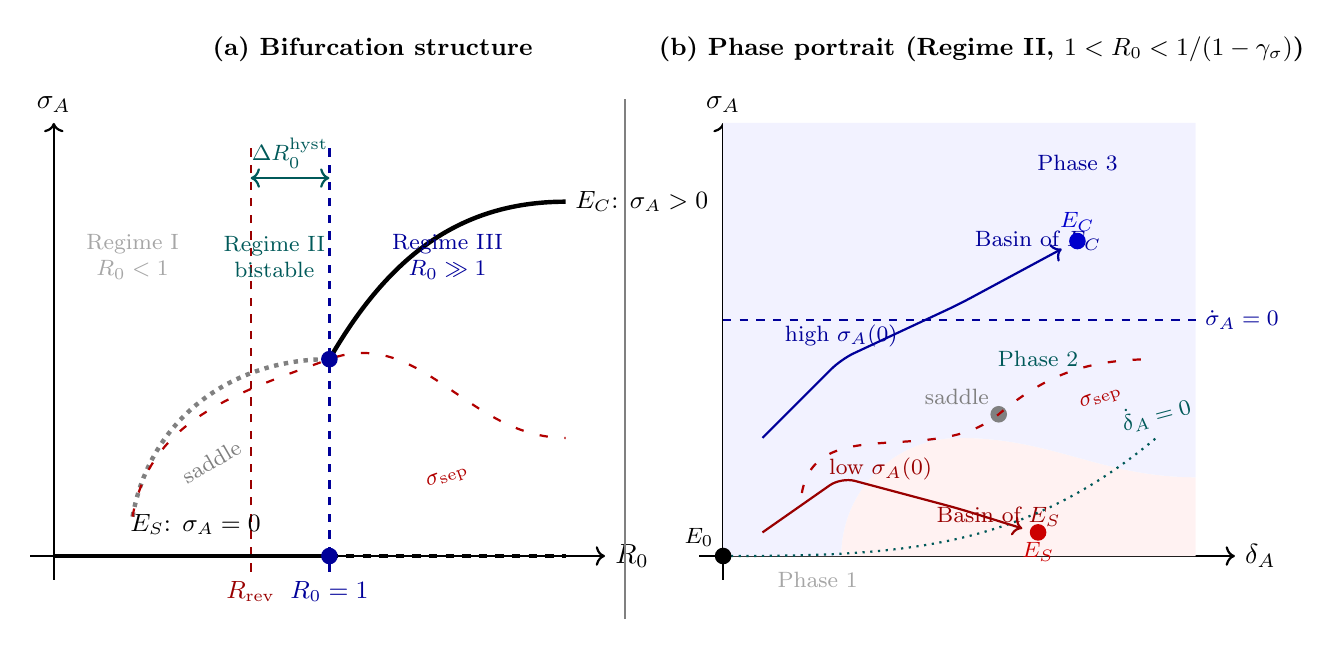
\begin{tikzpicture}[font=\sffamily]

    % ===== Panel (a): Bifurcation Diagram =====
    \begin{scope}[local bounding box=bifurcation]
        \draw[->, thick] (-0.3, 0) -- (7.0, 0) node[right] {$R_0$};
        \draw[->, thick] (0, -0.3) -- (0, 5.5) node[above] {$\sigma_A$};

        % R_0 = 1 line
        \draw[dashed, thick, blue!60!black] (3.5, -0.2) -- (3.5, 5.2);
        \node[below, font=\small, text=blue!60!black] at (3.5, -0.2) {$R_0 = 1$};

        % Reverse threshold R_rev
        \draw[dashed, thick, red!60!black] (2.5, -0.2) -- (2.5, 5.2);
        \node[below, font=\small, text=red!60!black] at (2.5, -0.2) {$R_{\mathrm{rev}}$};

        % Hysteresis band arrow
        \draw[<->, thick, teal!70!black] (2.5, 4.8) -- (3.5, 4.8);
        \node[above, font=\footnotesize, text=teal!70!black] at (3.0, 4.8) {$\Delta R_0^{\mathrm{hyst}}$};

        % Stable E_S branch (sigma=0, stable for R_0 < 1)
        \draw[ultra thick, black] (0, 0) -- (3.5, 0);
        \draw[ultra thick, black, dashed] (3.5, 0) -- (6.5, 0);
        \node[above, font=\small] at (1.8, 0.15) {$E_S$: $\sigma_A = 0$};

        % Unstable saddle branch
        \draw[ultra thick, black!50, dotted] (1.0, 0.5) to[out=80, in=180] (3.5, 2.5);
        \node[font=\footnotesize, text=black!50, rotate=30] at (2.0, 1.2) {saddle};

        % Bifurcating E_C branch (sigma > 0, stable for R_0 > 1)
        \draw[ultra thick, black] (3.5, 2.5) to[out=60, in=180] (6.5, 4.5);
        \node[right, font=\small] at (6.5, 4.5) {$E_C$: $\sigma_A > 0$};

        % Separatrix
        \draw[thick, red!70!black, loosely dashed] (1.0, 0.5) to[out=80, in=200] (3.5, 2.5)
            to[out=20, in=180] (6.5, 1.5);
        \node[font=\footnotesize, text=red!70!black, rotate=20] at (5.0, 1.0)
            {$\sigma_{\mathrm{sep}}$};

        % Label regimes
        \node[font=\footnotesize, text=gray!70, align=center] at (1.0, 3.8) {Regime I\\$R_0 < 1$};
        \node[font=\footnotesize, text=teal!70!black, align=center] at (2.8, 3.8) {Regime II\\bistable};
        \node[font=\footnotesize, text=blue!60!black, align=center] at (5.0, 3.8) {Regime III\\$R_0 \gg 1$};

        % Bifurcation point marker
        \fill[blue!60!black] (3.5, 2.5) circle (3pt);
        \fill[blue!60!black] (3.5, 0) circle (3pt);
    \end{scope}

    % ===== Panel (b): Phase Portrait (Regime II - bistable) =====
    \begin{scope}[local bounding box=portrait, shift={(8.5, 0)}]
        \draw[->, thick] (-0.3, 0) -- (6.5, 0) node[right] {$\delta_A$};
        \draw[->, thick] (0, -0.3) -- (0, 5.5) node[above] {$\sigma_A$};

        % E_S basin of attraction
        \fill[red!5] (0, 0) -- (1.5, 0) to[out=90, in=180] (3.0, 1.5)
            to[out=0, in=180] (6.0, 1.0) -- (6.0, 0) -- cycle;

        % E_C basin of attraction
        \fill[blue!5] (1.5, 0) to[out=90, in=180] (3.0, 1.5)
            to[out=0, in=180] (6.0, 1.0) -- (6.0, 5.5) -- (0, 5.5) -- (0, 0)
            -- (1.5, 0) -- cycle;

        % E_C basin label
        \node[font=\footnotesize, text=blue!60!black] at (4.0, 4.0) {Basin of $E_C$};
        \node[font=\footnotesize, text=red!60!black] at (3.5, 0.5) {Basin of $E_S$};

        % Nullclines
        % sigma nullcline
        \draw[thick, blue!60!black, dashed] (0, 3.0) -- (6.0, 3.0);
        \node[font=\footnotesize, text=blue!60!black, right] at (6.0, 3.0) {$\dot{\sigma}_A = 0$};

        % delta nullcline (approximate)
        \draw[thick, teal!70!black, dotted] (0, 0) to[out=0, in=220] (5.5, 1.5);
        \node[font=\footnotesize, text=teal!70!black, rotate=15] at (5.5, 1.8) {$\dot{\delta}_A = 0$};

        % Equilibria
        % E_0
        \fill[black] (0, 0) circle (3pt);
        \node[above left, font=\footnotesize] at (0, 0) {$E_0$};

        % E_S
        \fill[red!80!black] (4.0, 0.3) circle (3pt);
        \node[below, font=\footnotesize, text=red!80!black] at (4.0, 0.3) {$E_S$};

        % Saddle point
        \fill[black!50] (3.5, 1.8) circle (3pt);
        \node[above left, font=\footnotesize, text=black!50] at (3.5, 1.8) {saddle};

        % E_C
        \fill[blue!80!black] (4.5, 4.0) circle (3pt);
        \node[above, font=\footnotesize, text=blue!80!black] at (4.5, 4.0) {$E_C$};

        % Stable manifold (separatrix)
        \draw[thick, red!70!black, loosely dashed] (1.0, 0.8) to[out=80, in=220]
            (3.5, 1.8) to[out=40, in=180] (5.5, 2.5);
        \node[font=\footnotesize, text=red!70!black, rotate=20] at (4.8, 2.0)
            {$\sigma_{\mathrm{sep}}$};

        % Sample trajectory: falls to E_S
        \draw[->, thick, red!60!black, rounded corners=5pt]
            (0.5, 0.3) -- (1.5, 1.0) -- (3.0, 0.6) -- (3.8, 0.35);
        \node[font=\footnotesize, text=red!60!black] at (2.0, 1.1) {low $\sigma_A(0)$};

        % Sample trajectory: rises to E_C
        \draw[->, thick, blue!60!black, rounded corners=5pt]
            (0.5, 1.5) -- (1.5, 2.5) -- (3.0, 3.2) -- (4.3, 3.9);
        \node[font=\footnotesize, text=blue!60!black] at (1.5, 2.8) {high $\sigma_A(0)$};

        % Phase labels
        \node[font=\footnotesize, text=gray!70] at (1.2, -0.3) {Phase 1};
        \node[font=\footnotesize, text=teal!70!black] at (4.0, 2.5) {Phase 2};
        \node[font=\footnotesize, text=blue!60!black] at (4.5, 5.0) {Phase 3};
    \end{scope}

    % ===== Panel separator =====
    \draw[gray, thick] (7.25, -0.8) -- (7.25, 5.8);

    % ===== Panel labels =====
    \node[above, font=\small\bfseries] at ([yshift=2mm]bifurcation.north)
        {(a) Bifurcation structure};
    \node[above, font=\small\bfseries] at ([yshift=2mm]portrait.north)
        {(b) Phase portrait (Regime II, $1 < R_0 < 1/(1-\gamma_\sigma)$)};

\end{tikzpicture}

\caption{
  (a) Bifurcation structure of the fast subsystem as a function of $R_0$,
  showing the $\sigma$-trap branch $E_S$, the schema-coherent branch $E_C$,
  and the hysteresis band $\Delta R_0^{\mathrm{hyst}}$.
  (b) Phase portrait in the bistable Regime~II ($1 < R_0 < 1/(1-\gamma_\sigma)$),
  showing the basins of attraction of $E_S$ and $E_C$ separated by the
  stable manifold $\sigma_{\mathrm{sep}}$. Trajectories with initial
  $\sigma_A(0) > \sigma_{\mathrm{sep}}$ converge to $E_C$; those below
  fall to $E_S$.
}
\label{fig:phase-portrait}
\end{figure}

\begin{itemize}
\item \textbf{Phase 1 (Surface Learning).} $R_0 < 1$: all trajectories
  converge to $E_S$. Depth $\delta_A$ grows but schema coherence
  $\sigma_A$ remains at zero.
\item \textbf{Phase 2 (Schema Onset).} $R_0$ crosses 1: trajectories with
  $\sigma_A(0) > \sigma_{\mathrm{sep}}$ diverge from $E_S$ and converge
  to $E_C$. This is the critical phase transition.
\item \textbf{Phase 3 (Schema Consolidation).} $R_0 > 1$: the system is
  in the basin of $E_C$. Schema coherence continues to grow toward
  $\sigma^*_A$.
\item \textbf{Phase 4 (Schema Transfer).} $R_0 \gg 1$: $\sigma_A \to 1$
  (clamped). The system discovers intersection structures $\Psi_A > 0$.
\item \textbf{Phase 5 (Saturation).} $\sigma_A = 1$: maximal schema
  coherence. All cognitive faculties operate at ceiling.
\end{itemize}

The hysteresis band ensures that once Phase~3 is reached, the system
is robust to fluctuations in training conditions, consistent with the
companion paper's experimental observations.
